\section{Demonstrator Prototype}
\label{sec:prototype}
  

\subsection{High-Level View}
As any other machine learning project, this prototype learns how to predict the results of new data through the results of a given dataset with the results already set. As a consequence, we designed a prototype with a big input dataset of 6 Gb to test the technology. Implicitly the library is prepared for machine learning, the one used here, which is splitting, parallelizing and clustering when we use the data structure of this library call RDD.\\*

While processing, we are able to test the performance of Apache Spark and its component for machine learning, called MLLib. 
We check the differences in performance using the time spending in every training of a model because it has to compute a big amount of data, as consequence we can test this technology in terms about clustering and parallelizing huge amount of data and compare the results between native clustering and local clustering, by native we mean that we use the component by default with only one core for clustering and by local we mean to use the component with as many core as the machine has. There is a third one, called Remote Clustering, but it will not be discussed in this report.

\subsection{Implementation}

The following link contains the URL of the GitHub Repository of our project (Jupyter Notebook's and LaTex report's code):
\begin{center}
	\url{https://github.com/envilk/TaxisFareMLlibPyspark}\\*
\end{center}			
						
The project is implemented in a Jupyter Notebook (explained in section~\ref{sec:experiments}), in consequence the code is commented already between lines of code. That's why, the report follows with all the code of the prototype.
		
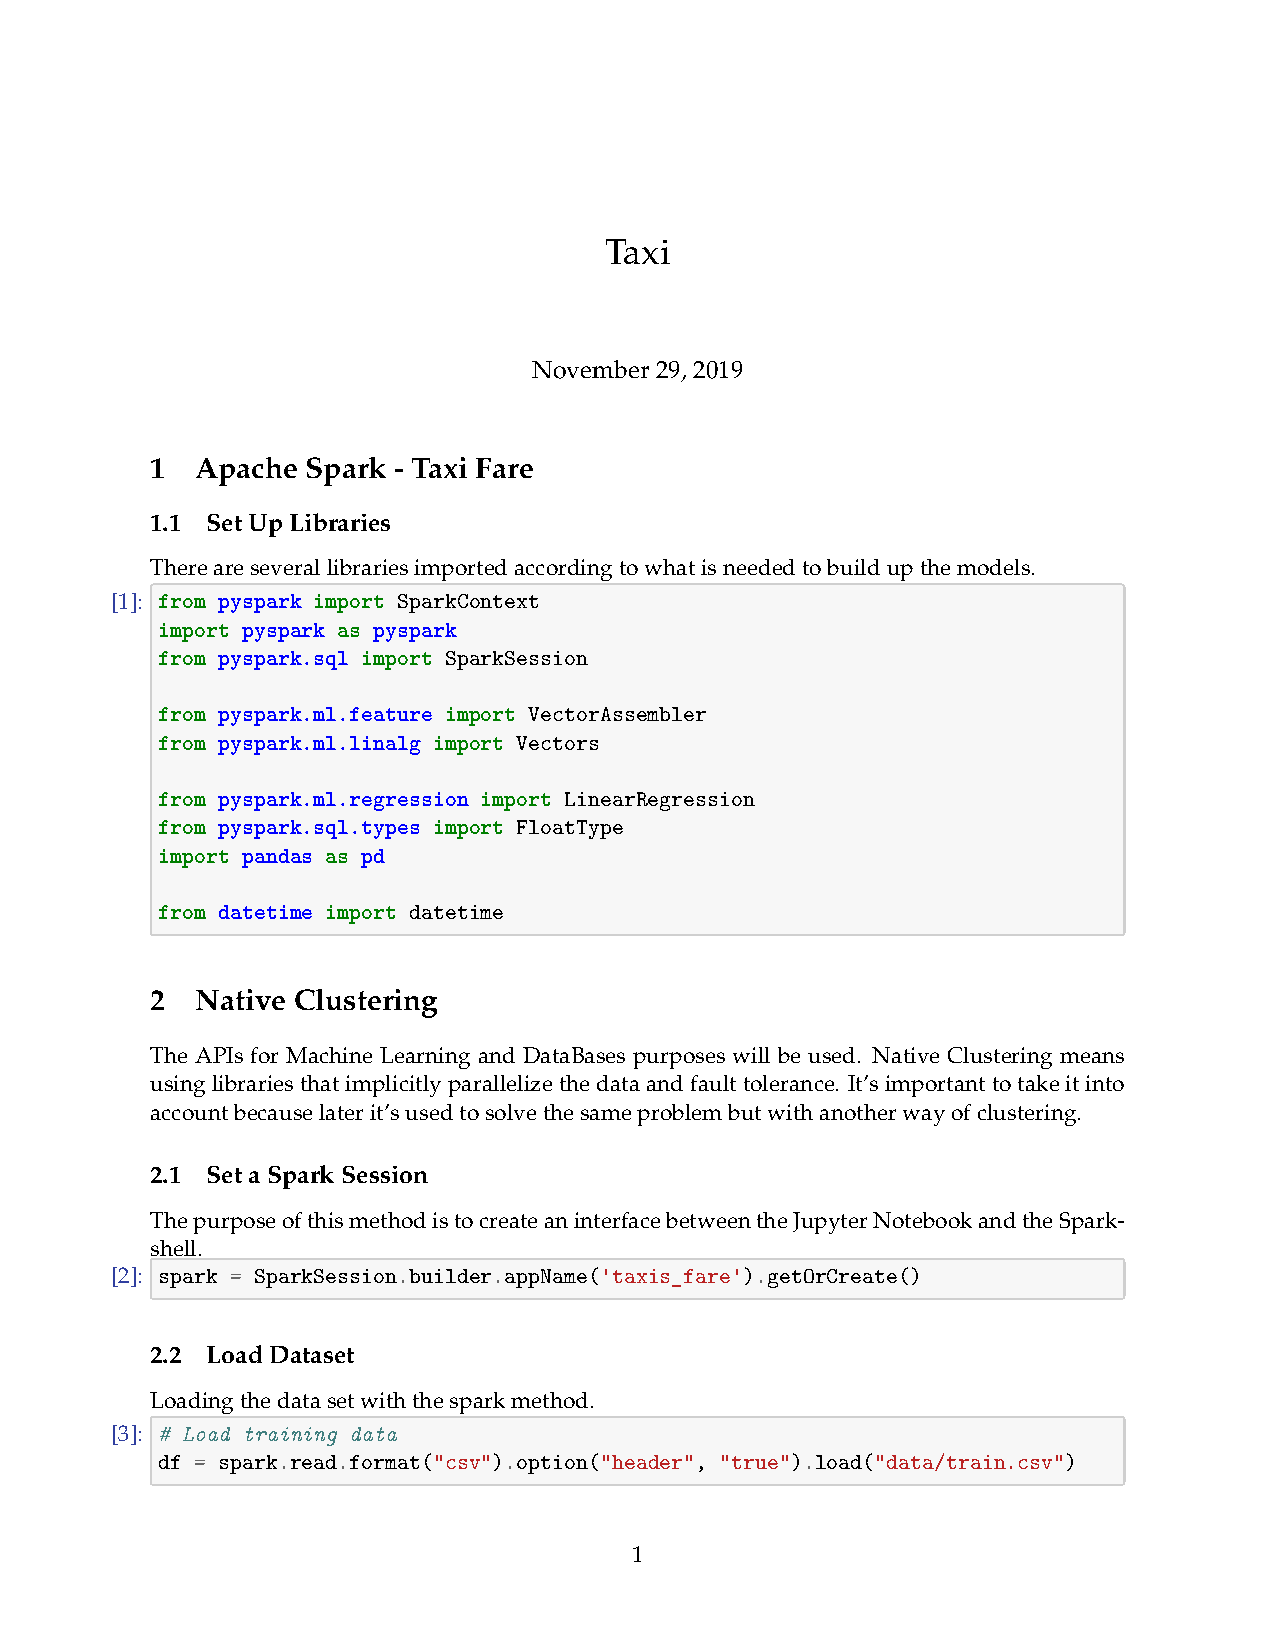
\includepdf[pages=1-11,scale=0.9]{code/Taxi.pdf}